\documentclass[../TDE7_ocrsf.tex]{subfiles}%

\begin{document}
\section[s]"2"{Résonance d'intensité dans un circuit RLC parallèle}

\enonce{%
	\noindent
	\begin{minipage}{0.60\linewidth}
		L'antenne d'un émetteur radio peut être modélisée par un circuit électrique
		équivalent composé de l'association en parallèle d'une résistance $R$,
		d'une bobine d'inductance $L$ et d'un condensateur de capacité $C$.
		\smallbreak
		L'antenne est alimentée par une source idéale de courant dont l'intensité
		caractéristique varie de manière sinusoïdale dans le temps: $i(t) = I_0
			\cos(\wt)$.
	\end{minipage}
	\hfill
	\begin{minipage}{0.35\linewidth}
		\begin{center}
			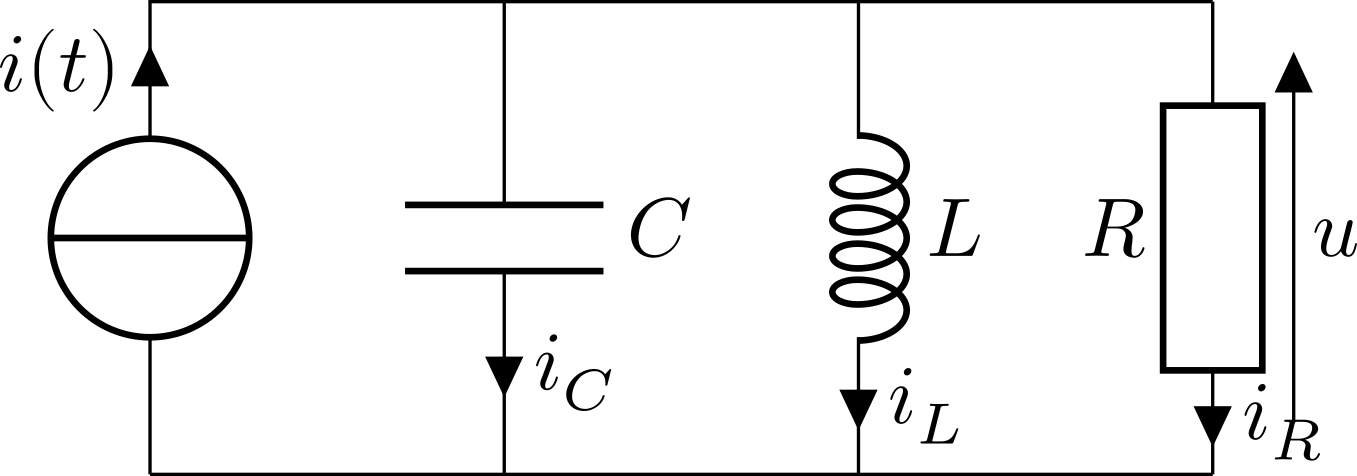
\includegraphics[width=\linewidth]{rlc_parr}
		\end{center}
	\end{minipage}

	On s'intéresse à la manière dont l'amplitude de la tension $u(t)$ aux
	bornes de l'antenne, qui correspond au signal envoyé, dépend de
	$\w$.
}

\QR{%
	Déterminer l'impédance complexe de l'association des dipôles $R,L$ et
	$C$.
}{%
	Soit $\Zu$ l'impédance équivalente à cette association, et $\Yu$ son
	admittance. On a
	\begin{gather*}
		\Yu = \frac{1}{R} + \frac{1}{\jlw} + \jcw
		= \frac{\jlw + R + (\jcw)R(\jlw)}{\jj RL\w}\\
		\Leftrightarrow
		\boxed{\Zu = \frac{\jj RL\w}{\jlw + R - RLC\w^2}}
	\end{gather*}
}

\QR{%
	En déduire l'amplitude complexe $\xul{U}$ de la tension $u$ en fonction
	de $\w$, $I_0$, $R$, $L$ et $C$.
}{%
	On a $\DS \frac{\Uu_0}{\Iu_0} = \Zu$ par définition de l'impédance,
	soit $\Uu_0 = \Zu\Iu_0 = \Zu I_0$ (étant donné que l'intensité n'a pas
	de phase à l'origine). Ainsi
	\begin{gather*}
		\Uu_0 = \frac{I_0\jj RL\w}{\jlw + R - RLC\w^2}
	\end{gather*}
	On rend cette équation plus lisible en mettant le dénominateur sous une
	forme adimensionnée en divisant par $\jlw$, ce qui donne
	\begin{gather*}
		\Uu_0 = \frac{RI_0}{1 + \dfrac{R}{\jlw} + \jj RC\w}
		\Leftrightarrow
		\boxed{\Uu_0 = \frac{RI_0}{1 + \jj \left( RC\w - \frac{R}{L\w} \right)}}
	\end{gather*}
}

\QR{%
	Pour quelle pulsation l'amplitude réelle $U$ de $u$ prend-elle sa
	valeur maximale notée $U_\text{max}$~? Conclure sur la fréquence à
	utiliser.
}{%
	L'amplitude réelle est
	\begin{gather*}
		U = \abs{\Uu_0} = \frac{RI_0}{\sqrt{1 + \left( RC\w - \dfrac{R}{L\w}
				\right)^2}}
	\end{gather*}
	Cette tension réelle est maximale si le dénominateur est minimal, donc
	si $\DS \left( RC\w - \frac{R}{L\w} \right) = 0$~: cela implique qu'il y
	a résonance si $\boxed{\w = \w_0 = 1/\sqrt{LC}}$. On trouve alors
	\begin{gather*}
		\boxed{U(\w_0) = U_{\max} = E_0}
	\end{gather*}
}

\QR{%
	Représenter le graphe donnant $U$ en fonction de la pulsation réduite
	$x=\w/\w_0$ avec $\w_0=1/\sqrt{LC}$.
}{%
	On cherche à faire apparaître $\w_0$ dans l'écriture de $U$~:
	\begin{align*}
		RC\w - \frac{R}{L\w}
		 & = R\w \frac{C\sqrt{L}}{\sqrt{L}} -
		\frac{R}{\w}\frac{\sqrt{C}}{\sqrt{C}L}
		 & = R\w \sqrt{\frac{C}{L}} \frac{1}{\w_0} -
		\frac{R}{\w} \sqrt{\frac{C}{L}} \w_0
		 & = R \sqrt{\frac{C}{L}} \left( x - \frac{1}{x} \right)
	\end{align*}
	En nommant $Q = \DS R \sqrt{\frac{C}{L}}$, on obtient finalement
	\begin{gather*}
		\boxed{\Uu_0 = \frac{RI_0}{1+\jj Q \left( x - \dfrac{1}{x} \right)}}
		\qsoit
		\boxed{U = \frac{RI_0}{\sqrt{1 + Q^2\left( x - \dfrac{1}{x}
					\right)^2}}}
	\end{gather*}
	On trace pour différentes valeurs de $Q$, et on obtient~:
	\begin{center}
		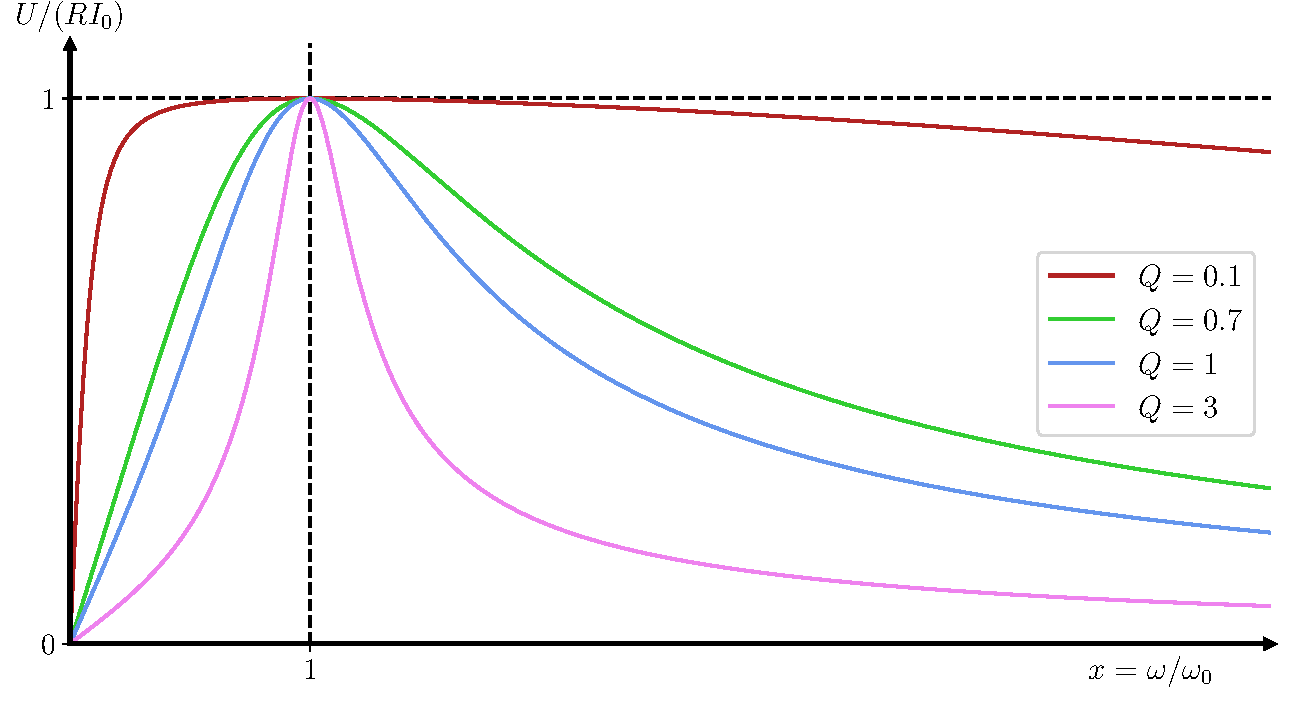
\includegraphics[width=.8\linewidth]{rlc_parr_U_ampl}
	\end{center}
}

\QR{%
	Exprimer la largeur de la bande passante $\Delta\w$.
}{%
	On cherche donc les pulsations de coupure telles que $U(\w) =
		\frac{U_{\max}}{\sqrt{2}}$, soit
	\begin{gather*}
		U(\w) = \frac{U_{\max}}{\sqrt{2}}
		\Leftrightarrow
		\frac{RI_0}{\sqrt{1 + Q^2\left( \dfrac{\w}{\w_0} - \dfrac{\w_0}{\w}
				\right)^2}}
		=
		\frac{RI_0}{\sqrt{2}}
		\Leftrightarrow
		\boxed{Q^2\left( \frac{\w}{\w_0} - \frac{\w_0}{\w} \right)^2 = 1}
	\end{gather*}
	On prend la racine carrée de cette équation, \textbf{en prenant les deux
		solutions possibles}~:
	\begin{align*}
		Q\left( \frac{\w}{\w_0} - \frac{\w_0}{\w} \right) = -1
		         & \qet
		Q\left( \frac{\w}{\w_0} - \frac{\w_0}{\w} \right) = 1          \\
		\Leftrightarrow
		\left( \frac{\w}{\w_0} - \frac{\w_0}{\w} \right)\times \w\w_0 =
		- \frac{\w\w_0}{Q}
		         & \qet
		\left( \frac{\w}{\w_0} - \frac{\w_0}{\w} \right)\times \w\w_0 =
		\frac{\w\w_0}{Q}                                               \\
		\Leftrightarrow
		\w^2 - \w_0{}^2 = -\frac{\w\w_0}{Q}
		         & \qet
		\w^2 - \w_0{}^2 = \frac{\w\w_0}{Q}                             \\
		\Leftrightarrow
		\boxed{
			\w^2 + \frac{\w_0}{Q}\w - \w_0{}^2 = 0}
		         & \qet
		\boxed{
		\w^2 - \frac{\w_0}{Q}\w - \w_0{}^2 = 0}                        \\
		\Rightarrow
		\Delta = & \frac{\w_0{}^2}{Q} + 4\w_0{}^2                      \\
		\Leftrightarrow
		\Delta = & \frac{\w_0{}^2}{Q^2} \left( 1 + 4Q^2 \right)        \\
		\Rightarrow
		\w_{1,\pm} = -\frac{\w_0}{2Q} \pm \frac{\w_0}{2Q} \sqrt{1+4Q^2}
		         & \qet
		\w_{2,\pm} = \frac{\w_0}{2Q} \pm \frac{\w_0}{2Q} \sqrt{1+4Q^2} \\
		\Leftrightarrow
		\w_{1,\pm} = \frac{\w_0}{2Q} \left(-1 \pm \sqrt{1+4Q^2}\right)
		         & \qet
		\w_{2,\pm} = \frac{\w_0}{2Q} \left(1 \pm \sqrt{1+4Q^2}\right)
	\end{align*}
	De ces quatre racines, seules deux sont positives~: la solution avec $-1 -
		\sqrt{1+4Q^2}$ est évidemment négative, et celle avec $1 - \sqrt{1+4Q^2}$
	également. Ainsi, il ne nous reste que
	\begin{gather*}
		\w_1 = \frac{\w_0}{2Q} \left( \sqrt{1+4Q^2}-1 \right)
		\qet
		\w_1 = \frac{\w_0}{2Q} \left( \sqrt{1+4Q^2}+1 \right)
	\end{gather*}
	Il ne reste qu'à calculer la différence pour avoir la bande passante~:
	\begin{gather*}
		\boxed{\D\w = \w_2 - \w_1 = \frac{\w_0}{Q}}
	\end{gather*}
}

\QR{%
	On se place dans le cas $R = \SI{7}{\Omega}$, $L = \SI{1.2e-8}{H}$ et $C =
		\SI{2.3e-10}{F}$. Calculer la valeur de l'acuité $A_c = \w_0/\Delta\w$
	de la résonance. Interpréter sa dépendance en $R$.
}{%
	$\w_0/\D\w$ est directement $Q$, donc on a
	\begin{gather*}
		A_c = Q = R \sqrt{\frac{C}{L}}
		\qavec
		\left\{
		\begin{array}{rcl}
			R & = & \SI{7}{\Omega}  \\
			L & = & \SI{1.2e-8}{H}  \\
			C & = & \SI{2.3e-10}{F}
		\end{array}
		\right.\\
		\mathrm{A.N.~:}\quad
		\boxed{A_c = \num{5.2}}
	\end{gather*}
	L'acuité augmente avec la résistance~: c'est normal puisque la
	résistance est en parallèle du circuit, donc une absence de résistance
	signifie ici $R$ infinie (pour qu'aucun courant ne la traverse).
}
\end{document}
